\documentclass[12pt,oneside]{book}
\newcommand{\TITLE}{Python}
\newcommand{\francais}{0}
\newcommand{\status}{0}
\newcommand{\lcheck}{0}
\newcommand{\more}{Based on AUB course EECE230X,\\
Note that most of the notes are copied from the AUB course pdf}
\newcommand{\yeare}{2022-2023}
\usepackage[utf8]{inputenc}
\usepackage[margin=0.5in]{geometry}
\usepackage[usestackEOL]{stackengine}
\usepackage{amsmath , esint,braket,lmodern,mhchem,bohr,lewis,chemfig,draftwatermark,xcolor,graphicx , amssymb ,ragged2e , listings , siunitx , float , eqparbox, centernot , esvect , bm , fancyhdr , fourier-orns}
\usepackage[ddmmyyyy]{datetime}
\usepackage{fourier-orns}
\usepackage{changepage}
\usepackage{bbm}\usepackage{chngcntr}
\usepackage{hyperref}
\usepackage{ifthen}
\usepackage[many]{tcolorbox}
\DeclareMathOperator{\sech}{sech}
\DeclareMathOperator{\csch}{csch}
\DeclareMathOperator{\arcsec}{arcsec}
\DeclareMathOperator{\arccot}{arcCot}
\DeclareMathOperator{\arccsc}{arcCsc}
\DeclareMathOperator{\arccosh}{arcCosh}
\DeclareMathOperator{\arcsinh}{arcsinh}
\DeclareMathOperator{\arctanh}{arctanh}
\DeclareMathOperator{\arcsech}{arcsech}
\DeclareMathOperator{\arccsch}{arcCsch}
\DeclareMathOperator{\arccoth}{arcCoth} 
\DeclareMathOperator{\grad}{\vv{\text{grad}}} 
\DeclareMathOperator{\conj}{^*} 
\DeclareMathOperator{\vect}{vv} 
\DeclareMathOperator{\Vect}{\text{Vect}} 
\DeclareMathOperator{\degree}{c^\circ} 
\DeclareMathOperator{\degre}{^\circ} 
\DeclareMathOperator{\transpose}{^\dagger} 
\DeclareMathOperator{\adjoint}{^\dagger} 

\newcommand{\moyenne}[1]{\langle #1 \rangle} 
\newcommand{\lagrange}{\mathcal{L}}
\newcommand{\fourier}{\mathcal{F}}
\newcommand{\hilbert}{\mathcal{H}}
\newcommand{\p}{\mathcal{P}}
\newcommand{\x}{\chi}
\newcommand{\ve}[1]{\vv{#1}}
\newcommand{\push}[1]{\begin{adjustwidth}{5mm}{}#1\end{adjustwidth}}
\newcommand{\operator}[1]{\widehat{#1}}
\newcommand{\HRule}{\rule{\linewidth}{0.5mm}} % Defines a new command for the horizontal lines, change thickness here
\renewcommand{\chaptermark}[1]{\markboth{\MakeUppercase{#1}}{}}
\renewcommand{\headrule}{%
\vspace{-8pt}\hrulefill
\raisebox{-2.1pt}{\quad\decofourleft\decotwo\decofourright\quad}\hrulefill}
\definecolor{myred}{RGB}{255, 14, 0}
\everymath{\displaystyle}

\def\changemargin#1{\list{}{\leftmargin#1}\item[]}
\let\endchangemargin=\endlist 

\makeatletter
\newcommand*{\rom}[1]{\expandafter\@slowromancap\romannumeral #1@}%roman numbers
\makeatother

%hyperlink shit

\hypersetup{
    colorlinks,
    citecolor=black,
    filecolor=black,
    linkcolor=black,
    urlcolor=black
}
% Table specail cell , it's for making line break in table cell
\newcommand{\specialcell}[2][c]{%
  \begin{tabular}[#1]{@{}c@{}}#2\end{tabular}}

  \definecolor{main}{HTML}{5989cf}    % setting main color to be used
\definecolor{sub}{HTML}{cde4ff}     % setting sub color to be used

\tcbset{
    sharp corners,
    colback = white,
    before skip = 0.2cm,    % add extra space before the box
    after skip = 0.5cm      % add extra space after the box
}   
\newtcolorbox{boxH}{
    colback = sub, 
    colframe = main, 
    boxrule = 0pt, 
    leftrule = 6pt % left rule weight
}
\newtcolorbox{gpt}{
    sharpish corners, % better drop shadow
    boxrule = 0pt,
    toprule = 4.5pt, % top rule weight
    enhanced,
    fuzzy shadow = {0pt}{-2pt}{-0.5pt}{0.5pt}{black!35} % {xshift}{yshift}{offset}{step}{options} 
}
\definecolor{codegreen}{rgb}{0,0.6,0}
\definecolor{codegray}{rgb}{0.5,0.5,0.5}
\definecolor{codepurple}{rgb}{0.58,0,0.82}
\definecolor{backcolour}{rgb}{0.95,0.95,0.92}

\lstdefinestyle{mystyle}{
    backgroundcolor=\color{backcolour},   
    commentstyle=\color{codegreen},
    keywordstyle=\color{magenta},
    numberstyle=\tiny\color{codegray},
    stringstyle=\color{codepurple},
    basicstyle=\ttfamily\footnotesize,
    breakatwhitespace=false,         
    breaklines=true,                 
    captionpos=b,                    
    keepspaces=true,                 
    numbers=left,                    
    numbersep=5pt,                  
    showspaces=false,                
    showstringspaces=false,
    showtabs=false,                  
    tabsize=2,
    basicstyle = \small
}

\lstset{style=mystyle}
\SetWatermarkAngle{45} 
\SetWatermarkLightness{.99} 
\SetWatermarkFontSize{0.1cm} 
\SetWatermarkScale{0} 
\SetWatermarkText{supahaka}


\begin{document}
\pagestyle{fancy}
\fancyhf{}
\fancyfoot[R]{Tenji$_\text{org}$}
\fancyfoot[C]{\thepage}
\fancyfoot[L]{\tiny www.tenji.org}
\fancyhead[RO]{\nouppercase{\leftmark\hfill\TITLE}}


\DraftwatermarkOptions{stamp=false}
    \begin{titlepage}
        \begin{center}
            \vspace*{5cm}
            \Huge
            \HRule \\[0.4cm]
            \textbf{Project Tenji: \\ \TITLE}\\
            \Large 
            \HRule \\[1.5cm]
            \vspace{2cm}
            \vfill
        \end{center}
        \vfill
        { \scriptsize Project Tenji \copyright 2024 by Khalil Salahat and Mohamad El Moussawi  \\}
        { \scriptsize Hosted at tenji.org , contact : contact@tenji.org \\}
        { \scriptsize \NOTICEE  \\}
    \end{titlepage} 
    \tableofcontents
\DraftwatermarkOptions{stamp=true}
\chapter{Getting Started}
An algorithm for a given problem is a list of instructions which given an input produces a desired output.
\section{Find square root }
\subsection{The problem }
given a nonnegative number x (the input), approximate its square root.\\
Interested in an approximation $g$ of $\sqrt{x}$ such that $g*g$ is close enough to $x$
\subsection{The algorithm}
Algorithm due to Heron of Alexandria, around 2000 years ago:
\begin{itemize}
	\item input : $x$ and tolerance parameter $\theta >0$
	\item start with a guess $g>0$
	\item if $g*g$ is close enough to $x$ ( $|g*g-x|\leq \theta$ ) stop.
	\item Else update $g$ to the value : $(g+\frac{x}{g})/2$
	\item Repeat until $|g*g - x| \leq \theta$
	\item Output : $g$
\end{itemize}
\pagebreak
\section{Search for a number in a sorted list }
\subsection{The problem}
Assume that you have a large list of $n$ numbers sorted  in non-decreasing order.\\
Given a number $x$, check if $x$ is in the list: YES/NO answer.
\subsection{Binary search algorithm}
Taking advantage of the fact that the numbers are sorted:
\begin{itemize}
	\item Compare $x$ to the middle element in the list
	\item if equal:\\
	      Stop and output :Yes
	\item if $x>$ middle:\\
	      narrow down search to upper sub-list excluding middle
	\item if $x>$ middle:\\
	      narrow down search to lower sub-list excluding middle
	\item Repeat until :\\
	      $x$ is found \\
	      or the sub-list is empty, in which case output:No
\end{itemize}
\section{Binary representation}

Binary digit (bit) : 0 or 1 \\
Byte: sequence of 8 bits\\
In general, using $n$ bits,  get $2^n$ combinations, thus for 8bits, we have $2^8 = 256$ combinations.\\

In Base 2 representation of integers we use 0 and 1:
\[ x_kx_{k-1}\dots x_0 = x_k\times10^k+x_{k-1}\times 10^{k-1}+\dots+x_0\times 10^0 \]
Example: $1100\to1\times2^3 + 1\times2^2 + 0\times 2^1+0\times 2^0 = 12$\\

In Base 10 representation of integers we use 0,1,2,3,4,5,6,7,8,9\\
\[ x_kx_{k-1}\dots x_0 = x_k\times2^k+x_{k-1}\times 2^{k-1}+\dots+x_0\times 2^0 \]
\chapter{Introduction to Python}
\section{Data Types}
Python is an interpreter, it guesses the type of a variable from initialization.
\subsection{int type}
used to represent integers.
\begin{lstlisting}[language=python]
m = 4 
n = 123124453654535612
p = -234
...
\end{lstlisting}
\subsection{float type}
Used to represent real number up to limited precision.\\
Represented using 8 bytes (64 bits) :
\begin{itemize}
	\item 1 bit for the sign $s$
	\item 52 bits the significant part $b$
	\item remaining $11$ bits for the exponent $e$ to put the floating decimal point
\end{itemize}
\[ (-1)^s \times 1.b\times 2^{\text{offset} - e} \]
\begin{lstlisting}[language=python]
f =24.2345
k=-56.45322342
...
\end{lstlisting}
\subsection{Bool type}
Used to represent Boolean/logical values: True and False
\begin{lstlisting}[language=python]
a = True
b = (8>3)
c = False 
...
\end{lstlisting}
\subsection{String type str}
It a sequence of characters\\
Use single quotations or double quotations
\begin{lstlisting}[language=python]
s = "ab d"
c = 'ab d'
\end{lstlisting}
Escape sequences:\\
\begin{tabular}{|l|l|l|l|l|}
	\hline
	Escape sequences       & Meaning      \\ \hline
	$\backslash$n          & New line     \\ \hline
	$\backslash$"          & "            \\ \hline
	$\backslash$'          & '            \\ \hline
	$\backslash\backslash$ & $\backslash$ \\ \hline
\end{tabular}
\subsection{Casting between types}
\begin{itemize}
	\item To integer\\
	      int(x) function: casts x to integer when possible.
	      \begin{lstlisting}[language=python]
int("12") #12
int(13.7) #13
int(True) # 1
\end{lstlisting}
	\item to float \\
	      float() function: casts to float when possible
	      \begin{lstlisting}[language=python]
float("-14.3") # -14.3 
\end{lstlisting}
	\item to string \\
	      str() function: cast to string
	      \begin{lstlisting}[language=python]
str(-1432.2) # "-1432.2"
\end{lstlisting}
\end{itemize}

\section{Operators}
\subsection{Arithmetic operators}
\subsubsection{Operators for the int and float types}
\begin{itemize}
	\item Addition (+) : $x+y$
	\item subtraction (-) : $x-y$
	\item Multiplication (*) : $x\times y$
	\item Division (/) : $\frac{x}{y}$
	\item Power (**) : $x^y$
\end{itemize}
All the above are binary operator: $x <\text{operator}> y \to z$\\
We have also a unary operator minus(-): $-x$ is the negative of $x$\\
Except of division if x and y are integer then the result in an integer,in all other cases the results are a float
\subsubsection{Operators specific to the int type}
\begin{itemize}
	\item Integer Division (//):\\
	      x//y is the quotient of x/y if y $\not = $ 0, (5//2 is 2)
	\item Modulo (\%): x\%y is the remainder of x/y, (5\% 2 is 1)
\end{itemize}
\subsection{Relational operators}
\begin{itemize}
	\item Equality check (==)
	\item Not equal (!=)
	\item Less than ($<$)
	\item Greater than ($>$)
	\item Less than or equal ($<=$)
	\item Greater than or equal ($>=$)
\end{itemize}
\subsubsection{Comparing two floats}
\begin{lstlisting}[language=python]
    x =0.1
    y = x*x # 0.010000000000000002
    x*x ==0.001# False 
    # use instead 
    abs(x*x -0.01) <= 1E-6
\end{lstlisting}
\subsection{Logical operators}

\begin{minipage}{0.3\linewidth}
	\begin{tabular}{|l|l|l|l|l|}
		\hline
		x     & y     & x and y \\ \hline
		True  & False & False   \\ \hline
		True  & True  & True    \\ \hline
		False & True  & False   \\ \hline
		False & False & False   \\ \hline
	\end{tabular}
\end{minipage}
\begin{minipage}{0.3\linewidth}
	\begin{tabular}{|l|l|l|l|l|}
		\hline
		x     & y     & x or y \\ \hline
		True  & True  & True   \\ \hline
		True  & False & True   \\ \hline
		False & True  & True   \\ \hline
		False & False & False  \\ \hline
	\end{tabular}
\end{minipage}
\begin{minipage}{0.3\linewidth}
	\begin{tabular}{|l|l|l|l|l|}
		\hline
		x     & not x \\ \hline
		True  & False \\ \hline
		False & True  \\ \hline
	\end{tabular}
\end{minipage}
\subsection{String operators}
\begin{itemize}
	\item Concatenation\\
	      using the + operator, ("abc" +"mnr" gives "abcmnr")
	\item Repetition\\
	      using the * operator,(3*"abc" gives "abcabcabc")
	\item length:
	      a build in function len(),(len("abc") gives 3)
\end{itemize}
\subsection{Order of precedence}
if we skip parentheses in an expression, the following order of precedence will be followed:\\
\begin{tabular}{|l|l|l|l|l|}
	\hline
	1 & Power : **                                    \\ \hline
	2 & Unary operator minus: -                       \\ \hline
	3 & Multiplication, division, modulo: *,/, // ,\% \\ \hline
	4 & Addition,Subtraction:+,-                      \\ \hline
	5 & Relational: $<,>,\leq,\geq,==,!=$             \\ \hline
	6 & not                                           \\ \hline
	7 & and                                           \\ \hline
	8 & or                                            \\ \hline
\end{tabular}
\section{Variables and the assignment operator}
In Python, a variable is just a name associated with an object. \\
In python, variables can change type:
\begin{lstlisting}[language=python]
    x =12.1 # float 
    x = "abc" string
\end{lstlisting}
\subsection{Naming variable}
A variable can't start with a digit, can't contain a spaces or symbols \\
It is recommended to capitalize first letter of each word except for initial word (secondNumber)\\
or separate by underscores (second\_number)
\section{Miscellaneous}
\subsection{Input}
Use input() function which returns a string.\\
Then, use the functions int() or float() functions to cast if needed
\begin{lstlisting}[language=python]
c = float(input('Enter a float: '))
\end{lstlisting}
\section{Output}
Use the function print(), which takes one or more arguments:
\begin{lstlisting}[language=python]
print(expression1,expression2,...)
\end{lstlisting}
\subsection{Modules}
Here some useful scientific modules:
\begin{itemize}
	\item math
	\item numpy : Numerical Python
	\item scipy: scientific tools for python
	\item matplotlib : 2D plotting library
\end{itemize}
\subsection{Comments}
Comments are ignored by python :
\begin{itemize}
	\item Starting a line with the hash symbol \# comments....
	\item Docstring """ comments.... """
\end{itemize}

\chapter{Selection and Repetition}
Selection and repetition flow diagrams:
\begin{center}
	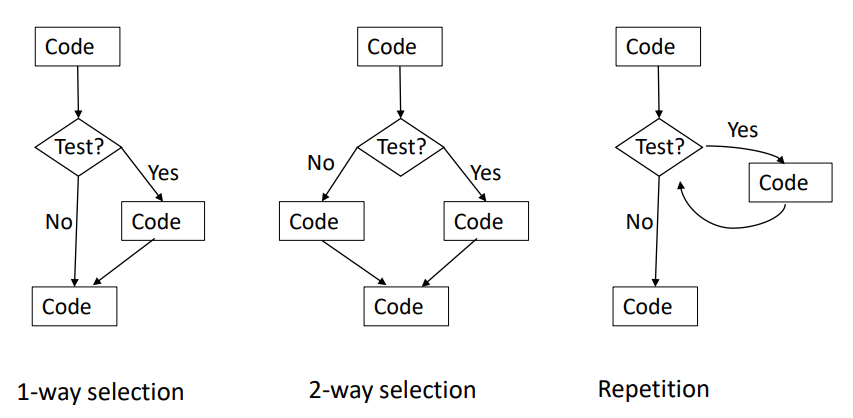
\includegraphics[width=0.5\linewidth]{../pic/python/25.png}
\end{center}
\section{Selection}
\subsection{if Structure}
Enables the program to branch depending on conditions.\\
Syntax :
\begin{lstlisting}[language=python]
if (Boolean expression):
    block of code 
\end{lstlisting}
The block has one ore more statements.\\
If the Boolean expression evaluates to True, the block is executed. Otherwise it is bypassed.

\subsection{if-else structure}
\begin{lstlisting}[language=python]
if Boolean expression:
    Block 1 of code 
else:
    Block 2 of code
\end{lstlisting}
If the Boolean expression evaluates to True, the first block is executed.\\
Otherwise, the second block is executed
\pagebreak
\subsection{Multi-way selection}
The two following syntax are equivalent :\\
\begin{minipage}{0.5\linewidth}
	The First one:
	\begin{lstlisting}[language=python]
if Boolean expression 1:
	Block 1 of code 
elif Boolean expression 2:
	Block 2 of code 
elif Boolean expression 3:
	Block 3 of code 
... 
else:	
	Block k of code 
\end{lstlisting}
\end{minipage}
\begin{minipage}{0.5\linewidth}
	The Second one:
	\begin{lstlisting}[language=python]
if Boolean expression 1:
	Block 1 of code 
else: 
	if Boolean expression 2:
		Block 2 of code 
	else :
		if Boolean expression 3:
			Block 3 of code 
		... 
				else :
					Block k of code
\end{lstlisting}
\end{minipage}
\section{Repetition: While loops and counters}
\subsection{while loop}
Enables the program to repeat a task as long as a condition is satisfied.\\
Syntax:
\begin{lstlisting}[language=python]
while Boolean expression:
	block of code
\end{lstlisting}
As long as the Boolean expression evaluates to True, the loop body is executed.
\subsection{Incrementing counters}
Incrementing an integer variable can be done by
\begin{lstlisting}[language=python]
i+=num # equivalent to i = i+num
\end{lstlisting}
\subsection{For loops}
Used to simplify syntax of counter controlled while loop:
\begin{lstlisting}[language=python]
variable = start 
while variable < stop:
	code block 
	variable = variable + step
\end{lstlisting}
For-loop syntax:
\begin{lstlisting}[language=python]
for variable in range(start,stop,step):
	code block
\end{lstlisting}
The default step is 1 and the default value of start is 0.
\subsection{break statement}
break statement : terminates the loop in which it is contained, and transfer control to the code immediately following the loop.\\
In nested loops, a break statement in the inner loop only affects the inner loop.\\
\section{Bisection method,Finding square-root}
\begin{itemize}
	\item Assume that $ x \leq 1 $
	\item We know that $\sqrt{x}$ is in the interval $[x,1]$
	\item Compute mid = (x+1)/2
	\item Compare mid*mid with x
	\item if abs(mid*mid-x)$\leq$ epsilon,stop
	\item if mid*mid$<$x, narrow down search to the interval [mid,1]
	\item Else, narrow down search to the interval [x,mid]
	\item Repeat the above process until abs(mid*mid -x)$\leq$ epsilon
\end{itemize}




\chapter{List,tuples,and strings}
\section{List type}
\subsection{Motivation}
Using what we know so far (scalar types, selection, and repetition), we can solve problems such as:
\begin{itemize}
	\item given a sequence of numbers
	\item find sum
	\item average
	\item max
\end{itemize}
But fall short of basic problems such as: given a sequence of numbers entered by user:
\begin{itemize}
	\item print them in reverse order
	\item check if they are distinct
	\item sort them
\end{itemize}
In all above three problems, we need to store all the sequence in memory and manipulate it,to do that we need lists.
\subsection{List type in python}
\begin{itemize}
	\item List is a built-in type :mutable (can be modified) ordered sequence of values, where each value is identified by an index
	\item Initialization:
\begin{lstlisting}[language=python]
L = [10,2,"ab",4.4]
\end{lstlisting}
	\item indexing:
\begin{lstlisting}[language=python]
L[i] # is the i'th element of L
\end{lstlisting}
	      the indexing start from zero
	\item length function
\begin{lstlisting}[language=python]
len(L) returns the length of L
\end{lstlisting}
	\item Read and Write
\begin{lstlisting}[language=python]
v=L[1] # stores the value of L[1] in v 
L[1]=7 # modifies the value of L[1]
\end{lstlisting}
	\item Homogenous lists : all elements are of the same type
	\item Non-homogenous lists: mixed types
\end{itemize}
\section{Manipulating lists}
\subsection{Initializing}
\begin{itemize}
	\item if n is an integer, the statement
\begin{lstlisting}[language=python]
L = [value]*n
\end{lstlisting}
creates a length-n list L whose entries are all of equal to value.
	\item Manipulating lists using loops
	      \begin{lstlisting}[language=python]
n = len(L)
for i in range(n)
	# proccess L[i]
\end{lstlisting}
	\item The range -n,...,-1 is special:
\begin{lstlisting}[language=python]
L[-1] #is interpreted as L[n-1]
\end{lstlisting}
\end{itemize}
\subsection{Input to list}
\begin{itemize}
	\item Method 1:
\begin{lstlisting}[language=python]
n = int(input("Enter number n of integers:"))
L = [0]*n 
for i in range(n):
	L[i] = int(input("Enter integer:"))
print(L)
\end{lstlisting}
	\item Method 2:
\begin{lstlisting}[language=python]
st = input("Enter integers separated by spaces:")
L=st.split()
for i in range(len(L)):
	L[i] = int(L[i])
print(L)
\end{lstlisting}
\end{itemize}
\subsection{The input reverse problem}
\begin{lstlisting}[language=python]
st = input("Enter integers separated by spaces: ")
L = st.split()
for i in range(len(L)):
	L[i] = int(L[i])
n = len(L)
for i in range(n-1,-1,-1):
	print(L[i],end=' ')
\end{lstlisting}
\section{Element distinctness problem}
Given a sequence of integers entered by user, check whether or not they are distinct
\begin{lstlisting}[language=python]
st = input("Enter integers separated by spaces: ")
L = st.split()
for i in range(len(L)):
	L[i] = int(L[i])
n = len(L)

distinct = True 
for i in range(n-1):
	for j in range(i+1,n):
		if L[i] ==L[j]:
			distinct = False 
			break 
	if not distinct: 
		break 
if(distinct):
	print("Elements are distinct")
else:
	print("Element not distinct")
\end{lstlisting}
\section{List copy}
\begin{itemize}
	\item The assignment operator on lists produces an alias:
\begin{lstlisting}[language=python]
L2 = Lchanging L, changes L2
\end{lstlisting}
	\item to get clone of L, use list.copy() method:
\begin{lstlisting}[language=python]
L3 =L.copy
\end{lstlisting}
\end{itemize}
\subsection{Reverse List}
\begin{itemize}
	\item WRONG SOLUTION:
	\begin{lstlisting}[language=python]
L = [1,2,15,20,17]
print(L)
n = len(L)
L2 = L
for i in range(n):
	L[i] = L2[n-1-i]
print(L)
	\end{lstlisting}
	since L2 is just an alias of L
	\item  We can use :
	\begin{lstlisting}[language=python]
L2 = L.copy() instead of L2 =L
\end{lstlisting}
Or :
\begin{lstlisting}[language=python]
L = [1,2,15,20,17]
print(L)
n = len(L)
for i in range (n//2):
	#swap L[i] and L[n-1-i]
	temp = L[i]
	L[i] = L[n-1-i]
	L[n-1-i] = temp 
print(L)
	\end{lstlisting}
	\item Or simply :
\begin{lstlisting}[language=python]
L.reverse()
\end{lstlisting}
\end{itemize}
\section{Tuples}
\begin{itemize}
	\item Tuples are immutable lists: once initialized cannot be modified, i.e., read-only
	\item Initialization: instead of brackets [] and commas as in lists, use parenthesis () and commas
\end{itemize}
\subsection{Application}
Swaping two variables :
\begin{lstlisting}[language=python]
(x,y) = (y,x)
\end{lstlisting}
Reverse problem:
\begin{lstlisting}[language=python]
for i in range(n//2):
	(L[i],L[n-1-i])=(L[n-1-i],L[i])
\end{lstlisting}
\subsection{Deep copy}
\begin{itemize}
	\item For a tuple T without mutable objects, only need the assignment operator T2 = T since anyways we cannot change T (there is no copy() method for type tuple).
	\item For a list containing mutable objects, the assignment operator L2=L creates an alias, and L2 = L.copy() creates a clone whose mutable objects are aliases.
	\item Deep copy: clone all mutable objects all the way, i.e., recursively.
\end{itemize}
\section{Sequences}
Sequence is an ordered set of objects, like:
\begin{itemize}
	\item lists
	\item tuples
	\item strings
	\item ranges
\end{itemize}
Strings are immutable, like tuples.\\
The indexing operators [i] can be used to access the i'th character of a string.
\subsection{Iterating over sequences}
L is a sequences
\begin{lstlisting}[language=python]
for x in L:
	code block to processes x 
    \end{lstlisting}
\section{List comprehension}
A concise way of initializing lists:
\begin{itemize}
	\item creates a list L consisting of the value of expression on x, for all elements x in the sequence.
\begin{lstlisting}[language=python]
L = [expression(x) for x in sequence]
\end{lstlisting}
	\item creates a list L consisting of the value of expression on x for all elements x in the sequence satisfying the condition.
\begin{lstlisting}[language=python]
L = [expression(x) for x in sequence if condition]
\end{lstlisting}
\end{itemize}
Examples:
\begin{lstlisting}[language=python]
L = [0 for i in range(5)] ===> [0,0,0,0,0]
L = [i for i in range(5)] ===> [0,1,2,3,4]
L = [i*i for i in range(5)] ===> [0,1,4,9,16]

mixed=[1,2,'a',3,4.0]
L = [x**2 for x in mixed if type(x) ==int] ===> [1,4,9]
\end{lstlisting}
\pagebreak
\chapter{Functions}
\section{Introduction}
A function has a name, input parameters (optional) , return value.\\
Why functions:
\begin{itemize}
	\item Abstraction
	\item Code decomposition
	\item Code reuse
\end{itemize}
\subsection{Defining new function}
{\small\begin{lstlisting}[language=python]
def functionName(formal parameters separated by commas):
	body of function
\end{lstlisting}}
if the function returns a value, the function body contains a return statement:
{\small\begin{lstlisting}[language=python]
return value
\end{lstlisting}}
and it may contain return statement to stop the execution of the function:
Calling the function:
{\small\begin{lstlisting}[language=python]
functionName(actual parameters separated by commas)
\end{lstlisting}}
\section{Scope of variables and execution stack}
Execution stack:
\begin{itemize}
	\item At function call, the actual parameters are assigned to the formal parameters
	\item The return statement stops the execution of the function and assigns the returned value
	\item Each function defines a new namespace, also called a scope
	\item Formal parameters and local variables exist only within the scope of the function’s definition
\end{itemize}
Scope of variables, Rules:
\begin{itemize}
	\item Variables are just names which refer to actual objects
	\item A variable cannot be used before being defined, i.e., initialized\\
	      Python guesses the type from initialization
	\item Initializing a variable in a function makes it a local variable in the function’s scope
\end{itemize}
\section{Functions handling lists,tuples,and strings}
Keep in mind that a variable of type list is just name which refers to an object of type list.\\
Passing a list to a function and returning a list from a function are done by the assignment operator: aliases are passed and returned, which is efficient\\
Example:
{\small\begin{lstlisting}[language=python]
def f(L):
	if len(L) >=1:
		L2 = [L[0],L[0]]
		L[0] = 0 
		L3 = L +L2 
		return L3 
	else: 
		return L 
A = [1,5,6] # it will change to [0,5,6]
B = f(A)  # [0,5,6,1,1]
\end{lstlisting}}
For strings and tuples they cannot be changed when passed as input arguments to functions, unless the tuples contain mutable objects.
\subsection{Python garbage collector}
Garbage collector: a process which eventually wakes up to clean up objects in memory that are not directly or indirectly accessible by variables.
after a function is called,it's local variable will be cleaned since they are not accessible in global scope.
\section{Miscellaneous}
\subsection{Building your own modules}
You can create a .py file that contain functions, and import those function by importing the .py file
{\small\begin{lstlisting}[language=python]
import myfunctions # for importing the file myfunctions.py in the same directory
\end{lstlisting}}
\subsection{Function defined in another function}
{\small\begin{lstlisting}[language=python]
def f(x):
	def g(y):
		return y+1 
	z = g(x)
	return z*z
\end{lstlisting}}
Here we can't call g from outside the function f
\subsection{Default parameters}
You can set default value for your formal parameters,the default value will be in place if the call of function didn't assign a value to it.
{\small\begin{lstlisting}[language=python]
def printName(firstName, lastName, reverse = False):
	if reverse:
		print(lastName + ', '+firstName)
	else: 
		print(firstName,LastName) 
printName("Homer","Simpson")#output: Homer Simpson 
printName("Homer","Simpson",True)#output: Simpson,Homer
\end{lstlisting}}
\subsection{Function without a return value}
Assigning a function which doesn't return value to a variable sets the variable's type to the None type
\section{Higher-order functions}
A function is called a higher-order function if:
\begin{itemize}
	\item it returns another function, or
	\item it takes another function as an input argument
\end{itemize}
\subsection{Functions are objects}
In python functions are objects, namely they maybe be:
\begin{itemize}
	\item passed to other functions
	\item returned by other functions
	\item assigned to variables
\end{itemize}
\subsection{Function taking another function as input argument}
{\small\begin{lstlisting}[language=python]
def linear(x):
	return x 
def square(x):
	return x*x  
def findsum(n,p):
	x=0 
	for i in range(1,n+1):
		x = x+p(i) 
	return x 
print(findSum(10,linear)) # output 55
print(findSum(10,square))# output 385
\end{lstlisting}}
\section{Some methods associated with list and str types}
\subsection{Methods associated with data types}
Types in python have methods associated with them.\\
T is a type and x is an object of type T.\\
we call those function by the member access operator " . "
\begin{itemize}
	\item list.copy
	\item list.reverse
	\item x.f(input parameters) , f is a member function of the type T
\end{itemize}
\subsection{List methods}
\begin{itemize}
	\item list.append(e):\\
		add object "e" to the end of the list it's the same as list = list + [e]\\
		it has no return value .\\
		Side effect:\\
		in the following example we get an infinite loop.
\begin{lstlisting}[language=python]
L = [1,20,3]
for e in L :
	L.append(e)
print(L)
\end{lstlisting}
	      L.append has an advantage over L = L+[e], which always creates a new list
	\item List.extend(L): adds the items in L to the end of List  \\
	      Has the same effect on L as L = L+L2 \\
	      it has no return value. \\
	      Same side effect as L.append
	\item L.count(e) returns the number of times that e occurs in L.
	\item L.insert(i,e) inserts the object e into L at index i.
	\item L.remove(e) deletes the first occurrence of e from L.
	\item L.index(e) returns the index of the first occurrence of e in L.
	\item L.pop(i) removes and returns the item at index i in L.
	\item L.sort() sorts the elements of L in ascending order
\end{itemize}
\subsection{Methods associated with the string type}
\begin{itemize}
	\item str.split : return the list of words for str \\
	      st.split(sep) will return the list of substring separated by sep
	\item List.join: return a string consisting of the strings in List \\
	      sep.join(L) will joint the elements of the list separated by sep
\end{itemize}
\chapter{Files and exceptions}
\section{Files}
Unlike lists , files are stored on drives.\\
\subsection{Manipulating files in python}
\subsubsection{General structure}
{\small\begin{lstlisting}[language=python]
nameHandle = open(fileName,mode)
nameHandle.close()#close the file
\end{lstlisting}}
\begin{itemize}
	\item fileName: string containing the path of the file
	\item mode:$\begin{cases}
			      \text{r: reading} \\
			      \text{w: writing} \\
			      \text{a: appending}
		      \end{cases}$
\end{itemize}
\subsubsection{Reading a file}
\begin{itemize}
	\item In one shot \\
	      \begin{lstlisting}[language=python]
nameHandle = open(fileName,'r')
s = nameHandle.read() # read the whole file into single string s
nameHandle.close()
\end{lstlisting}
	\item line by line\\
	      \begin{lstlisting}[language=python]
nameHandle=open(fileName,'r') 
for line in nameHandle:
	... 
nameHandle.close()
\end{lstlisting}
\end{itemize}
\subsubsection{Writing to a file}
{\small\begin{lstlisting}[language=python]
nameHandle = open(fileName,'w')
nameHandle.write(s)#now the file consists of the string s
#we can use the write method as many times as needed to append additional strings 
nameHandle.close()
\end{lstlisting}}
Note that if we open an existing file in the 'w' mode, its content will be disregarded,\\
if we want to write instead of overwriting we must use the mode 'a' instead of 'w'. \\
Note that if the file doesn't exist it will be created.\\
\subsection{Iterable versus subscriptable objects}
If we can iterate over object (for something in object ...) then the object is iterable.\\
when we can use an indexing operator with the object (object[i]) then the object is subscriptable.\\
The file object is iterable and not subscriptable.
\section{Exceptions and assertions}
Exception are something that does not conform to the norm.\\
we can handle exceptions.\\
Common exceptions:
\begin{itemize}
	\item TypeError (e/"abc")
	\item IndexError (L=["a,","b,"] and try to accessL[2])
	\item ValueError (int("abc"))
	\item ZeroDevisionError
	\item FileNotFoundError
\end{itemize}
\subsection{Handling exceptions}
\subsubsection{Try-except statement}
Instead of program crashing, Code Block B will execute if an exception is raised in Code Block A.
For any error:
{\small\begin{lstlisting}[language=python]
try:
	Code Block A 
except:
	Code Block B 
\end{lstlisting}}
Or :
{\small\begin{lstlisting}[language=python]
try: 
	Code Block A 
except Error_1:
	Code Block B_1
except Error_k:#will execute only if Error_k was raised in Block A
	Code Block B_k 
except: #will execute if an exception other than all the above was raised in Block A
	Code Block B
\end{lstlisting}}
\subsection{Assertions}
The assert statement raises an AssertionError if the boolean expression was False.
{\small\begin{lstlisting}[language=python]
assert Boolean expression,"error message" 
\end{lstlisting}}
\chapter{Miscellaneous: plotting, randomness, and Monte Carlo simulation }
\section{Plotting}
\begin{itemize}
	\item Importing the plotting module :
\begin{lstlisting}[language=python]
import matplotlib.pyplot as plt
\end{lstlisting}
	\item Let X and Y be lists of numbers of the same length, representing x and y coordinates. \\
	      To plot $Y$ as a function of $X$,use
\begin{lstlisting}[language=python]
plt.plot(X,Y,color)
\end{lstlisting}
	      color is a string taking values such as "k" for black, "r" for red, "b" for blue ...\\
	      The plot function plots the points (X[i],Y[i]), for i = 0 ,...,len(X)-1\\
	      connected by lines of colors color.
	\item to include labels :
\begin{lstlisting}[language=python]
plt.xlabel("x label text")
plt.ylabel("y label text")
\end{lstlisting}
	\item to include a title, use
\begin{lstlisting}[language=python]
plt.title("title text")
\end{lstlisting}
	\item to show the figure
\begin{lstlisting}[language=python]
plt.show()
\end{lstlisting}
	\item to clear a figure
\begin{lstlisting}[language=python]
plt.clf()
\end{lstlisting}
	\item to plot on a new or existing figure whose index is i, use
\begin{lstlisting}[language=python]
plt.figure(i)
plt.close(i)#to close figure i
\end{lstlisting}
	\item To plot on the same figure multiple graphs with tiled axes, use
\begin{lstlisting}[language=python]
plt.subplot(m,n,i)
\end{lstlisting}
	      \begin{itemize}
		      \item m: number of rows
		      \item n: number of columns
		      \item i: graph index
	      \end{itemize}
	\item When plotting multiple functions on the same figure, it helps to include a legend to label the functions\\
	      you can add a label
\begin{lstlisting}[language=python]
plt.plot(X,Y,label="myLabel")
\end{lstlisting}
	it appears when you invoke :
\begin{lstlisting}[language=python]
plt.legend()
\end{lstlisting}
	\item If the y-values contain very large and very small numbers, use log scale on the y-axis:
\begin{lstlisting}[language=python]
plt.yscale('log')
\end{lstlisting}
\end{itemize}
\section{Generating random numbers}
\begin{itemize}
	\item Import the numerical python module numpy
\begin{lstlisting}[language=python]
import numpy.random as rand
\end{lstlisting}
	\item To generages a uniformly random number in the real interval [x,y]
\begin{lstlisting}[language=python]
rand.uniform(x,y)#float 
rand.randint(x,y)#int
\end{lstlisting}
\end{itemize}
\section{Monte Carlo Simulation}
Monte Carlo simulation is a technique used to approximate the probability of an event by random sampling multiple times, and averaging the results.
\subsection{Approximating $\pi$}

\begin{minipage}{0.7\linewidth}
	\begin{itemize}
		\item Area of unit circle : $\pi \times 1^2 = \pi$
		\item Area of unit square : $2\times 2 = 4$
		\item $\frac{\text{area of unit circle}}{\text{area of unit sqaure}} = \frac{\pi}{4}$
		\item Thus the probability $p$ that a random point of the unit square belongs to the unit circle is $\frac{\pi}{4}$\\
		      Which mean : $\boxed{\pi = 4\times p}$
	\end{itemize}
\end{minipage}
\begin{minipage}{0.3\linewidth}
	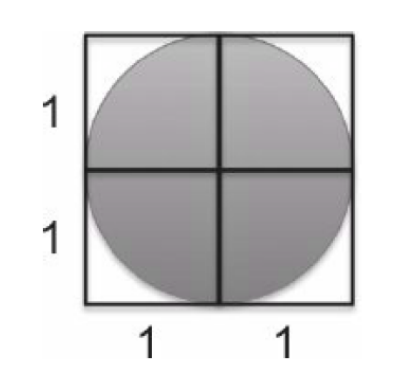
\includegraphics[width=\linewidth]{../pic/python/1.png}
\end{minipage}
Now to approximate $\pi$:
\begin{itemize}
	\item Choose n point (x,y) where x and y between -1 and 1
	\item Find the number m of points in the unit circle
	\item Return $\frac{4m}{n}$
	\item For large n, get an approximation of $\pi$
\end{itemize}
\chapter{Program efficiency,binary Search, insertion sort}
\section{Asymptotic Analysis: Theta notation}
\subsection{Linear search}
Consider the linear search
	{\small\begin{lstlisting}[language=python]
c1    def linearSearch(L,e):  
c2        n = len(L)
c3        i = 0 
c4        while i<n:
c5            if L[i] ==e:
c6                return i 
c7            i = i+1 
c8        return -1
\end{lstlisting}}
Let $T(n)$ is the wors case running time of linearSearch on a size-n list \\
The worst case if e not in L \\
Thus :\\
$T(n) = c_1 + c_2 + (c_4+c_5+c_7)\times n + c_4 + c_8= (\text{constant})\times n + (\text{negligable term compared to }n)$
\subsection{Asymptotic Analysis}
Its a solution to measure the running of algorithm.\\
we look at the growth of $T(n)$ as the input size $n\to\infty$\\
The keys are:
\begin{itemize}
	\item ignore constants
	\item ignore low order terms
\end{itemize}
\subsubsection{Theta notation}
Here it comme the Theta notation as following:
\begin{itemize}
	\item $5n+17 \implies \theta(n)$
	\item $6n^2+18n+5 \implies \theta(n^2)$
	\item $3\log(n) + 7\implies \theta(\log(n))$
	\item $10 \implies \theta{1}$
\end{itemize}
\underline{Definition:}\\
Let $f(n)$ and $g(n)$ be function defined on the nonnegative integers.\\
We say that $f(n) = \theta(g(n))$ if: $\boxed{\lim_{n\to\infty}\frac{f(n)}{g(n)} = a}$ a strictly positive constant.\\
More generally even if the limit doesn't exist, we say that $f(n) = \theta(g(n))$ if $f(n)$ can be sandwiched between two positive constant multiples of $g(n)$.\\
\[\boxed{ 0 \leq c_1 \times  g(n) \leq f(n) \leq c_2 \times g(n)}\]
\subsection{Working with Theta}
\subsubsection{Useful properties}
\begin{itemize}
	\item $f(n) = \theta(g(n))$ and $g(n) = \theta(h(n)) \implies f(n) = \theta(h(n))$
	\item $\theta(g(n)) + \theta(g'(n)) = \theta(g(n) + g'(n))$
	\item $\theta(g(n)) \times \theta(g'(n)) = \theta(g(n)\times g'(n))$
\end{itemize}
\subsubsection{Linear search running time}
Back to the linear search running time we can use theta notation as following: $T(n) = \theta(n)$ steps\\
For the best case running time : $\theta(1)$ (if L[0] ==e)\\
In case of searching for two elements (two sequential loops), the theta notation as following:\\
$\theta(n) + \theta(n) = \theta(n)$\\
Nesting loops costs more
\subsubsection{Naive distinct element algorithm}
{\small\begin{lstlisting}[language=python]
def naiveDistinctElements(L):
	n = len(L)
	for i in range(n):
		for j in range(n):
			if i!=j and L[i] ==L[j]:
				return False 
	return True 
\end{lstlisting}}
Theta notation : $\theta(1) + n\times(\theta(n)) = \theta(n^2)$ steps
\subsubsection{Better Distinct Elements algorithm}
{\small\begin{lstlisting}[language=python]
def distinctElements(L):    
	n = len(L)
	for i in range(n):
		for j in range(i+1,n):
			if L[i] ==L[j]:
				return False 
	return True
\end{lstlisting}}
Number of tests is reduced by half, but it is still quadratic
\subsubsection{Square tests}
By a naive square test : $\theta(\sqrt{n})$ arithmetic operations\\
By bisection:
{\small\begin{lstlisting}[language=python]
def isSquareBisection(n):
	if n<0: return False 
	elif n==0:return True  
	else: 
		low =1 
		high =n 
		while low <=high: 
			mid = (low+high)//2 
			if mid*mid ==n :
				return True 
			elif mid*mid<n:
				low = mid +1 
			else: 
				high = mid-1 
		return False
\end{lstlisting}}
it take $\theta(log(n))$ arithmetic operations.\\
because after each iteration, the lenght of the search interval is reduced by at least half
\subsubsection{Imporatant Note}
$\theta(n)$ arithmetic operations $\not = \theta(n)$ steps since:\\
for large n, multiplication operation in factorial algorithm costs is more than $\theta(1)$ step.
\section{Other asymptotic notations}
\begin{itemize}
	\item Theta : $ f(n) = \theta(g(n))$ \\
	      $f(n)$ is asymptotically like $g(n)$
	\item Big O: $f(n) = O(g(n))$\\
	      $f(n)$ is asymptotically like $g(n)$ or weaker than $g(n)$\\
	      There exist $c>0$ and $n_0 >0$ such that for all $n>n_0$,$0\leq f(n) \leq c\times g(n)$
	\item Little o: $f(n) = o(g(n))$\\
	      $f(n)$ is asymptotically weaker than $g(n)$\\
	      $\lim_{n\to \infty} \frac{f(n)}{g(n)} =0$
\end{itemize}
$f(n) = O(g(n))$ and $g(n) = O(f(n)) \longleftrightarrow f(n) = \theta(g(n))$
\subsection{Worst case running time}
\begin{itemize}
	\item $T(n) = \theta(g(n))$ mean that:\\
	      The worst case running time grows like $g(n)$.
	\item $T(n) = O(g(n))$ mean that:\\
	      The worst case running time grows like $g(n)$ or is weaker than $g(n)$.
	\item $T(n) = o(g(n))$ mean that:\\
	      The algorithm is asymptotically much faster than $g(n)$
\end{itemize}
\subsection{Common growth rates}
\begin{itemize}
	\item $\theta(1)$ called constant running time.
	\item $\theta(log(n))$ called logarithmic running time.
	\item $\theta(n)$ called linear running time.
	\item $\theta(nlog(n))$ is called log-linear running time.
	\item $\theta(n^2)$ is called quadratic running time.
	\item $\theta(n^k),k>0$ constant, is called polynomial running time.
	\item $\theta(c^n),c>1$ constant, is called exponential running time.
\end{itemize}
\begin{center}
	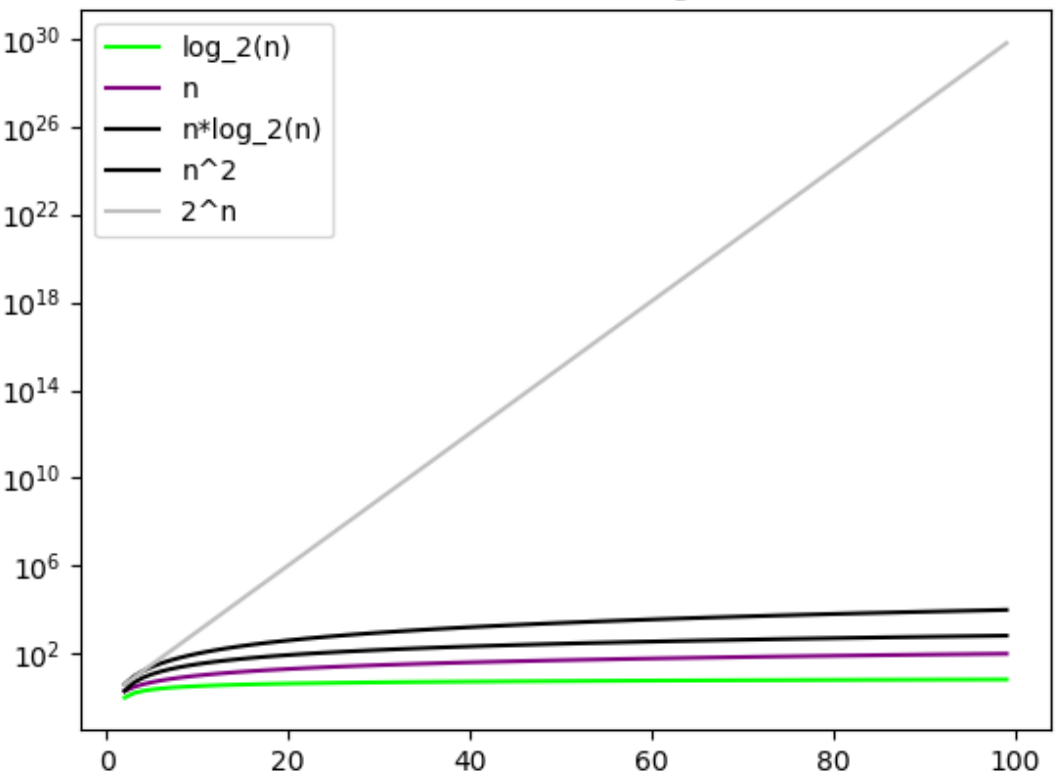
\includegraphics[width=0.5\linewidth]{../pic/python/2.png}
\end{center}
\section{Binary Search}
Well linear search takes linear time, we expect algorithm faster than linear search.
\subsection{The idea}
In a sorted list (in non-decreasing order), we want to find if x is in L and return its index if it exist.
\begin{itemize}
	\item Same as the bisection method
	\item Compare x with the middle element of L.
	\item if $>$, ignore the lower half of L including middle element of L since L is sorted.
	\item if $<$,ignore the upper half of L including middle element since L is sorted.
	\item if $=$, we are done ( x is an element of L).
	\item Repeat.
\end{itemize}
{\small\begin{lstlisting}[language=python]
def binarySearch(L,x):
	n = len(L)
	low =0 
	high = n-1 
	while low <=high:
		mid = (low+high)//2
		if L[mid] == x: 
			return mid 
		elif L[mid]<x: 
			low = mid+1 
		else:
			high = mid-1
	return -1
\end{lstlisting}}
The worst case running of binary search on a list of size n is $\theta(log(n))$ steps, less than $\theta(n)$.
\section{Sorting problem}
The selection sort algorithm take $\theta(n^2)$ time.\\
Now the insertion Sort, which also takes $\theta(n^2)$time.\\
\subsection{Insertion Sort}
Idea:
\begin{itemize}
	\item First element ok.
	\item Compare the second element with the first and insert in the correct place.
	\item Compare the third element with the second,and if needed with the first to insert it in the correct place.
	\item And so till the end
\end{itemize}
\begin{center}
	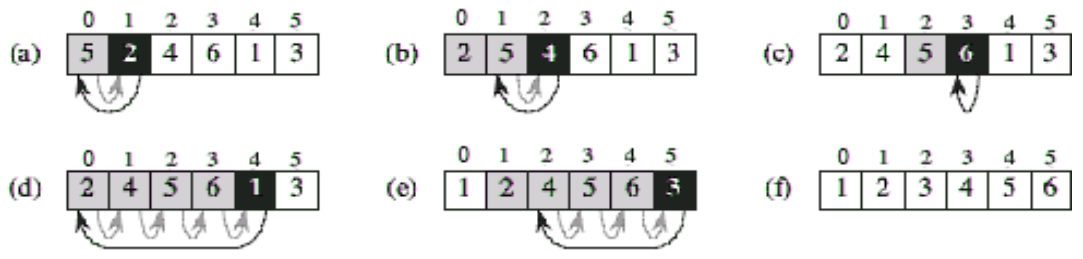
\includegraphics[width=0.4\linewidth]{../pic/python/3.png}
\end{center}
The code:
{\small\begin{lstlisting}[language=python]
def insertionSort(L):
	n = len(L)
	for j in range(1,n):
		key = L[j]
		i = j -1 
		while i >=0 and L[i] > key:
			L[i+1] = L[i]
			i = i -1 
		L[i+1] = key
\end{lstlisting}}
\subsubsection{Comparision slection versus insertion sort}
\begin{center}
	\begin{tabular}{|l|l|l|l|l|}
		\hline
		                                   & Selection Sort & Insertion Sort           \\
		\hline
		Worst case running time            & $\theta(n^2)$  & $\theta(n^2)$            \\
		\hline
		Best case running time             & $\theta(n^2)$  & $\theta(n)$              \\
		\hline
		Number of write operations on list & $\theta(n)$    & $\theta(n^2)$ Worst case \\ \hline
	\end{tabular}
\end{center}
\section{Time analysis of some list operations and methods}
\subsection{Some operations and methods}
\begin{tabular}{|l|l|l|l|l|}
	\hline
	Equality Check: L1==L2   & $\theta(len(L1)+len(L2))$ \\ \hline
	Concatenation: L = L1+L2 & $\theta(len(L)+len(L2))$  \\ \hline
	Membership: e in L       & $\theta(len(L))$          \\ \hline
	Slicing: L[i:j]          & $\theta(j-i)$             \\ \hline
	L.count(e)               & $\theta(len(L))$          \\ \hline
	L.index(e)               & $\theta(len(L))$          \\ \hline
	L.reverse()              & $\theta(len(L))$          \\ \hline
\end{tabular}
\subsection{List.append}
In the worst case $L.append(e)$ operations takes $\theta(len(L))$ time:\\
if not enough contiguous cells are available, the whole list is copied to new place in memory and resized.\\
The point is that when copied to a new place in memory, the list is resized to twice its size to allow for efficient append in the next iterations.\\
That mean copy will only happen when the list length is a power of 2:1,2,4,8,16...\\
Thus total cost is: $\boxed{\theta(n)}$.\\
While L = L+[e] method cost:$\theta(n^2)$ be cause for each iteration the cost of $L = L +[e]$ is $\theta(i)$ by creating new list.
\subsection{list.sort}
list.sort takes $\theta(nlog(n))$ time to sort a size-n list, much faster than selection sort and insertion sort,which take $\theta(n^2)$.
\chapter{Recursion}
\section{Introduction: recursive factorial and recursion stack}
A recursive definition defines a structure in terms of a smaller version of itself.\\
To stop the recursion, every recursive definition must have at least one base case.\\
The general case must eventually reduce the definition into the base case.\\

example: Factorial:recursive definition $\begin{cases}
		0! = 1: n=0 \text{ is the base case} \\
		n! = (n-1)!\times n \text{ if } n \geq 1 \text{: the general case}
	\end{cases}$\\
\begin{minipage}{0.6\linewidth}
	Code:
	\begin{lstlisting}[language=python]
def recursiveFactorial(n):
    if n == 0: return 1
    else:
        y = recursiveFactorial(n-1)
        return n*y 
print(recursiveFactorial(3))
\end{lstlisting}
\end{minipage}
\begin{minipage}{0.3\linewidth}
	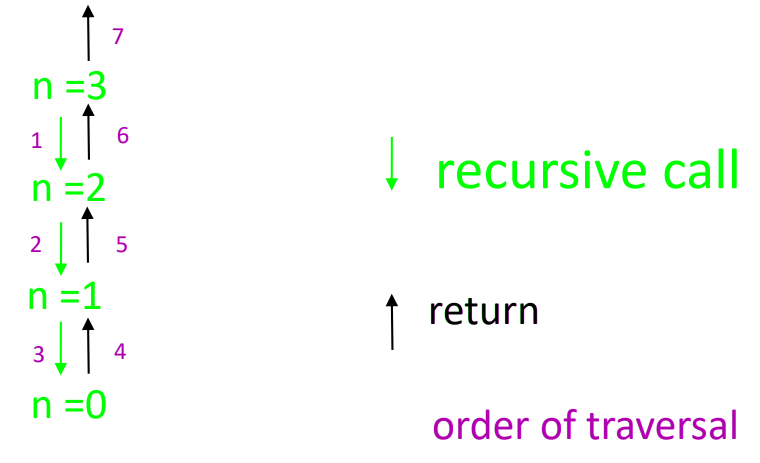
\includegraphics[width=\linewidth]{../pic/python/4}
\end{minipage}
\subsection{Recursion stack}
The recursion stack is the execution stack when recursion is involved \\
Each recursive call to a recursive function has its own:
\begin{itemize}
	\item parameters
	\item local variables
	\item return value
	\item control (knows where to return when done)
\end{itemize}
Remember that :\\
when a function call completes control returns to the calling function.\\
execution in the calling function resumes from the point immediately following the call.
\pagebreak
\subsection{Iterative Factorial}
{\small\begin{lstlisting}[language=python]
def iterativeFactorial(n):
    x =1 
    for i in range(1,n+1):
        x = x*i 
    return x 
print("iterativeFactorial(5):",iterativeFactorial(5))
\end{lstlisting}}
\subsection{Recursive versus iterative factorial}
\begin{minipage}{0.5\linewidth}
	Recursive:\\
	Time : $\theta(n)$ arithmetic operations \\
	Space : $\theta(N)$ integers
\end{minipage}
\begin{minipage}{0.5\linewidth}
	Iterative:\\
	Time : $\theta(n)$ arithmetic operations \\
	Space : $\theta(1)$ integers
\end{minipage}\\
iterative implementation is better.
\section{Tracking recursion, indirect recursion, infinite recursion}
\subsection{Order of printing}

\begin{minipage}{0.3\linewidth}
	Order 1 :\\
\begin{lstlisting}[language=python]
def f(n):
	print(n,end="")
	if n >=1:
		f(n-1)
f(10)
\end{lstlisting}
\end{minipage}
\begin{minipage}{0.1\linewidth}
	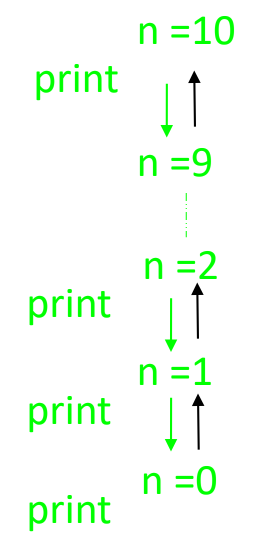
\includegraphics[width=\linewidth]{../pic/python/5}
\end{minipage}
\begin{minipage}{0.2\linewidth}
	.
\end{minipage}
\begin{minipage}{0.3\linewidth}
	Order 2 :\\
\begin{lstlisting}[language=python]
def g(n):
	if n >=1:
		f(n-1)
	print(n,end="")
g(10)
\end{lstlisting}
\end{minipage}
\begin{minipage}{0.1\linewidth}
	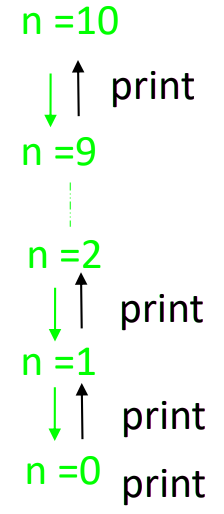
\includegraphics[width=\linewidth]{../pic/python/6}
\end{minipage}
\subsection{Infinite recursion}
Infinite recursion: every function call results in a recursive function call.\\
in theory it executes forever but the computer executes until it runs out of memory.\\
if not intended, it is usually the result of missing base case, or the problem does not reduce to the base case.
\subsection{Indirect recursion}
\begin{itemize}
	\item Direct recursion: a function calls itself
	\item Indirect recursion: a function f calls other functions that eventually end up calling f
\end{itemize}
\pagebreak
\section{Two-way recursion: Fibonacci numbers}
Two-way recursion: recursive function which calls itself twice, the key concept is recursion  tree.\\
\subsection{Fibonacci numbers}
\begin{itemize}
	\item Base case:
	      \begin{itemize}
		      \item $F_0 = 0$
		      \item $F_1 = 1$
	      \end{itemize}
	\item General case: \\
	      $F_n = F_{n-1} + F_{n-2}$ if $n \geq 2$
\end{itemize}
\begin{center}
	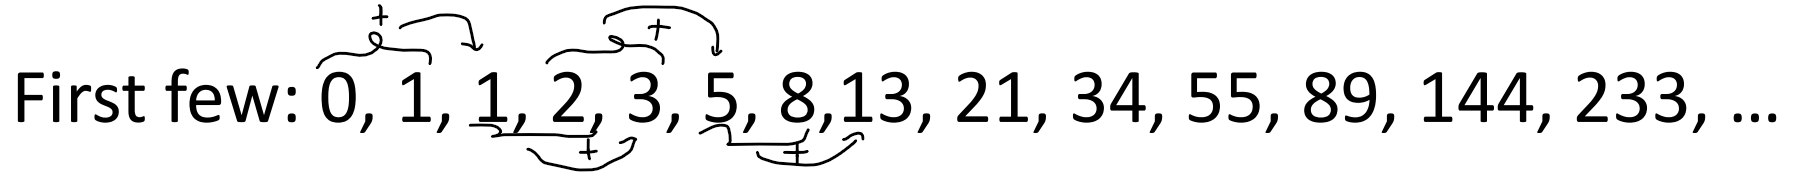
\includegraphics[width=0.7\linewidth]{../pic/python/7.png}
\end{center}
\subsection{Fibonacci numbers: recursive function}

\begin{minipage}{0.6\linewidth}
	\begin{lstlisting}[language=python]
def recFib(n):
    assert type(n) == int and n >=0, "bad input!"
    # the two base cases 
    if n ==0 or n==1: return n 
    else:
        prev1 = recFib(n-1)
        prev2 = recFib(n-2)
        return prev1 + prev2 # combine the results 
print(recFib(5))
\end{lstlisting}
\end{minipage}
\begin{minipage}{0.4\linewidth}
	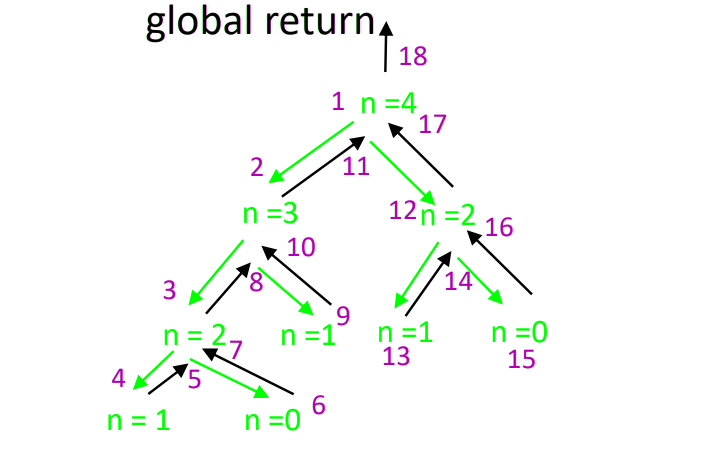
\includegraphics[width=\linewidth]{../pic/python/8}
\end{minipage}
\begin{tabular}{|l|l|l|l|l|l|l|l|l|l|l|l|l|l|l|l|l|l|l|l|l|l|l|l|l|l|}
	\hline
	Step:          & 1 & 2 & 3 & 4 & 5 & 6 & 7 & 8 & 9 & 10 & 11 & 12 & 13 & 14 & 15 & 16 & 17 & 18 \\ \hline
	Stack content: & 4 & 4 & 4 & 4 & 4 & 4 & 4 & 4 & 4 & 4  & 4  & 4  & 4  & 4  & 4  & 4  & 4  & 4  \\ \hline
	Stack content: &   & 3 & 3 & 3 & 3 & 3 & 3 & 3 & 3 & 3  &    & 2  & 2  & 2  & 2  & 2  &    &    \\ \hline
	Stack content: &   &   & 2 & 2 & 2 & 2 & 2 &   & 1 &    &    &    & 1  &    & 0  &    &    &    \\ \hline
	Stack content: &   &   &   & 1 &   & 0 &   &   &   &    &    &    &    &    &    &    &    &    \\ \hline
\end{tabular}\\

Recursion tree captures the recursion process of multi-way recursion.
\begin{itemize}
	\item Each node corresponds to a recursive call.
	\item Root: initial call
	\item Leaves: base cases
	\item Down arrows: recursive call
	\item Up arrow: return
\end{itemize}
\begin{minipage}{0.7\linewidth}
	Recursive function not efficient:
	\begin{itemize}
		\item It solves the same subproblem multiple times
		\item For instance, $F_3$ is computed twice and $F_2$ three times
	\end{itemize}
\end{minipage}
\begin{minipage}{0.3\linewidth}
	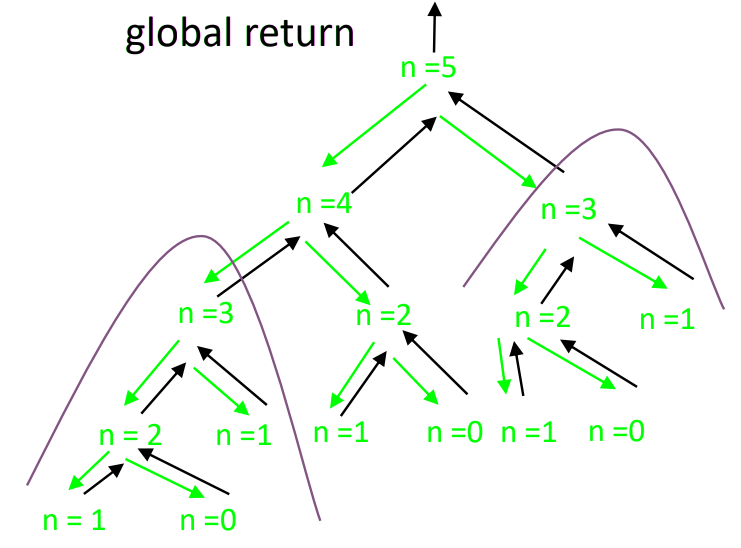
\includegraphics[width=\linewidth]{../pic/python/9}
\end{minipage}
recursive Fibonacci time $ = 2^{\theta(n)}$ arithmetic operations\\
recursive Fibonacci space $ = \theta(n)$
\subsection{Fibonacci numbers: non-recursive:list-based}
{\small\begin{lstlisting}[language=python]
def fibListBased(n):
    assert type(n) == int and n>=0,"Bad input!"
    L = [0]*(n+1)
    if n ==0 or n==1: return n 
    else:
        L[0] =0 
        L[1] =1 
        for i in range(2,n+1):
            L[i] = L[i-1]+L[i-2]
        return L[n]
\end{lstlisting}}
Time $\theta(n)$, space$\theta(n)$
\subsection{Fibonacci numbers: recursive: memoized}
Memoization: to avoid resolving previously solved problems, help recursion with look-up list L[0...n]
\begin{itemize}
	\item Initially all entries in list are -1
	\item Before resolving check list
	\item if -1, solve and save in list
	\item Else, return value in list
\end{itemize}
Memoization is an overkill for Fibonacci, but very useful for other problems

\begin{minipage}{0.5\linewidth}
	\begin{lstlisting}[language=python]
def FibMemoized(n):
    assert type(n) ==int and n>=0,"Bad input!"
    def recFibMemoized(n,L):
        if L[n] != -1:
            return L[n]
        elif n==0 or n==1:
            L[n] =n 
        else: 
            L[n] = recFibMemoized(n-1,L)+recFibMemoized(n-2,L)
        return L[n]
    L = [-1]*(n+1)
    return recFibMemoized(n,L)
\end{lstlisting}
\end{minipage}
\begin{minipage}{0.4\linewidth}
	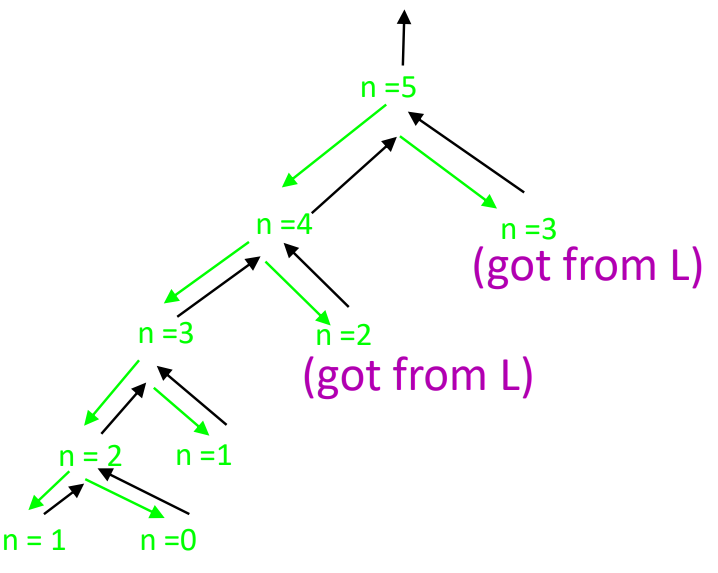
\includegraphics[width=\linewidth]{../pic/python/10}
\end{minipage}
Time $\theta(n)$ arithmetic operations , Space: $\theta(n)$ integers
\subsection{Fibonacci numbers: non-recursive O(1) space }
Key: enough to keep track of the last two Fibonacci numbers
	{\small\begin{lstlisting}[language=python]
def fib(n):
    assert type(n) ==int and n>=0,"Bad input!"
    if n==0 or n==1: return n 
    previous2 = 0 
    previous1 = 1
    for i in range(2,n+1):
        current = previous1+previous2 
        previous2 = previous1 
        previous = current 
    return current
\end{lstlisting}}
Time $\theta(n)$, space$\theta(1)$
\subsection{Better than $\theta(n)$ arithmetic operations}
key: matrix identity: for $n\geq 1$
\[  \left( \begin{matrix}
			1 & 1 \\
			1 & 0 \\
		\end{matrix}\right)^n =  \left( \begin{matrix}
			F_{n+1} & F_n     \\
			F_n     & F_{n-1} \\
		\end{matrix}\right)\]
\section{Two-way recursion: tower of Hanoi}
\subsection{Tower of Hanoi problem}

\begin{minipage}{0.6\linewidth}
	\begin{itemize}
		\item Given 3 needles and n disks of increasing size.
		\item The n disks are originally stacked on needle 1 in increasing size with largest at the bottom.
		\item Target is to move the disks to needle 3 and place in the same same order.
		\item Constraints:
		      \begin{itemize}
			      \item Move one disk at a time from one needle to another
			      \item A disk can not be placed on top of a smaller disk.
		      \end{itemize}
	\end{itemize}
\end{minipage}
\begin{minipage}{0.4\linewidth}
	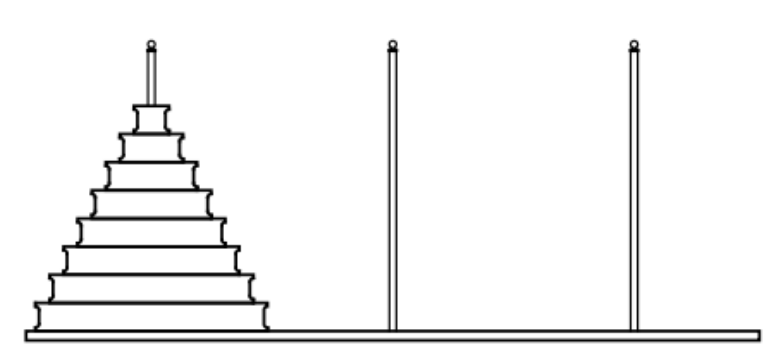
\includegraphics[width=\linewidth]{../pic/python/11}
\end{minipage}
\subsubsection{Solution}

\begin{minipage}{0.6\linewidth}
	To move n disks from needle 1 to needle 3:
	\begin{itemize}
		\item 1. if $n\geq 2$, move top $n-1$ disks recursively from needle 1 to needle 2, using needle 3 as an intermediate needle.
		\item 2.Move disk from needle 1 to needle 3
		\item 3. if $n\geq 2$,move top $n-1$ disks recursively from needle 2 to needle 3, using needle 1 (which is now empty) as an intermediate needle.
	\end{itemize}
\end{minipage}
\begin{minipage}{0.4\linewidth}
	For n =3\\
	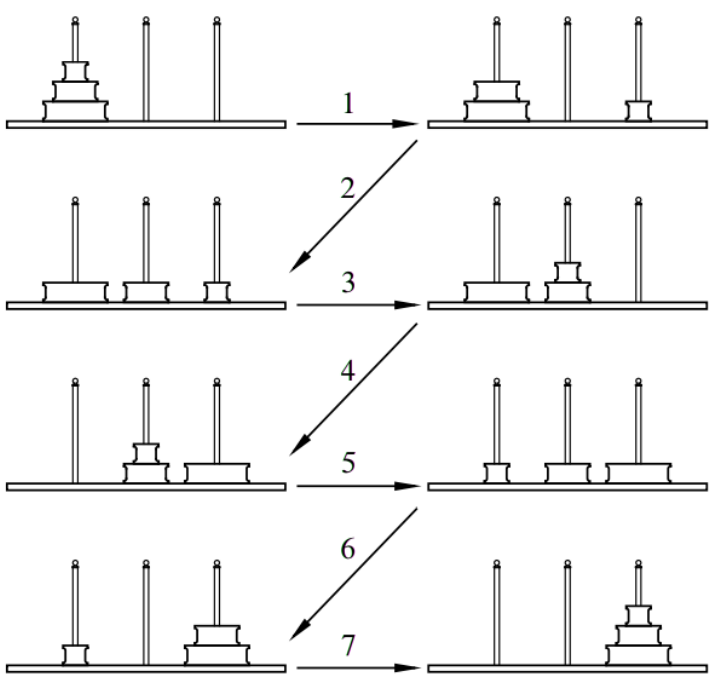
\includegraphics[width=\linewidth]{../pic/python/12}
\end{minipage}
Base case : $n=1$ do second step only.\\

\begin{minipage}{0.6\linewidth}
	Code:
	\begin{lstlisting}[language=python]
def moveDisks(n,start=1,destination=3,intermediate=2):
    if n>=2:
        moveDisks(n-1,start,intermediate,destination)
    print("Move disk",n,"from",start," to ",destination)
    if n >=2:
        moveDisks(n-1,intermediate,destination,start)
moveDisks(3)
\end{lstlisting}
\end{minipage}
\begin{minipage}{0.4\linewidth}
	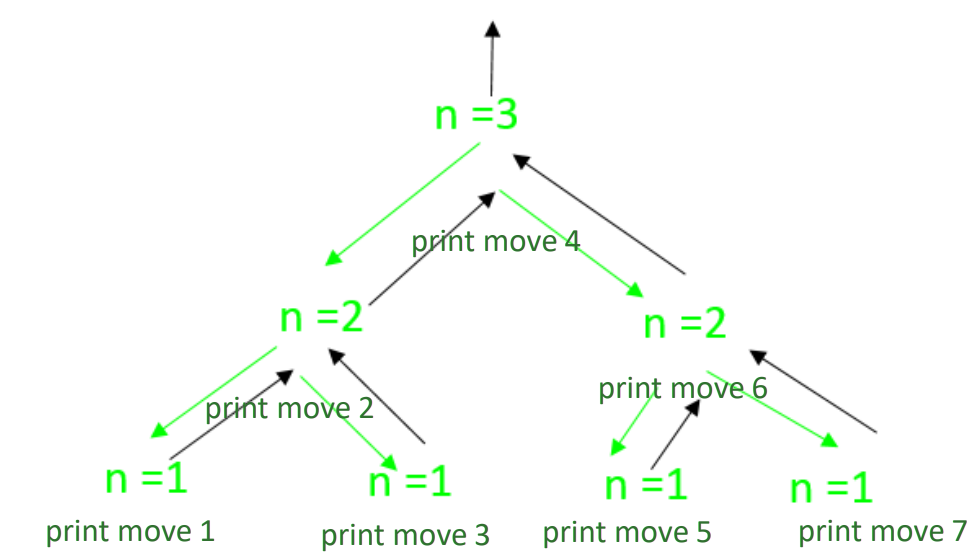
\includegraphics[width=\linewidth]{../pic/python/13}
\end{minipage}
Time : $\theta(2^n)$,sapce $\theta(n)$
\section{Recursive binary search}
\subsection{Recursive viewpoint}
To find the index of x in a sorted list L:
\begin{itemize}
	\item Compare middle element of L with x
	\item If $=,$ return index of middle element
	\item If $<,$ recur on the upper half of L
	\item If $>,$ recur on the lower half of L
	\item If recursive call is on empty list, return -1
\end{itemize}
Base case: two base cases 2 and 5
\subsection{Implement the recursiveBinarySearch function}
Don’t pass lower half or upper half as slices to the function as slicing makes copies and the this takes linear time \\
Instead, pass the indices low and high in addition to L (just an alias) and x, which takes constant time:
{\small\begin{lstlisting}[language=python]
def search(L,x):
    def recBinarySearch(L,x,low,high):
        if low>high:return -1
        mid = (low+high)//2
        if L[mid] ==x:
            return mid 
        elif L[mid]<x:
            return recBinarySearch(L,x,mid+1,high)
        else:
            return recBinarySearch(L,x,low,mid-1)
    return recBinarySearch(L,x,0,len(L)-1)

\end{lstlisting}}
\subsection{Iterative versus recursive binary search}

\begin{minipage}{0.5\linewidth}
	Iterative binary search :\\
	Time $\theta(log(n))$ steps \\
	Space $\theta(1)$
\end{minipage}
\begin{minipage}{0.5\linewidth}
	Recursive binary search \\
	Time $\theta(log(n))$ steps \\
	Space $\theta(log(n))$
\end{minipage}\\
iterative best.

\chapter{Data structures digression}
Data structures are used to store and manage data.\\
Dynamic sets are data structures that support certain operations, also called queries, such as search, insert, and delete.
\section{Lists of lists}
A list L of lists is a list whose entries are objects of type list.\\
\subsection{Representing graphs using lists of lists}
Adjacency list representation of graph:

\begin{minipage}{0.6\linewidth}
	Adj[i] is a list containing the nodes adjacent to node i:
\begin{lstlisting}[language=python]
Adj = [[1,2],[2,3],[1,3,4],[1,4],[],[4]]
\end{lstlisting}
\end{minipage}
\begin{minipage}{0.4\linewidth}
	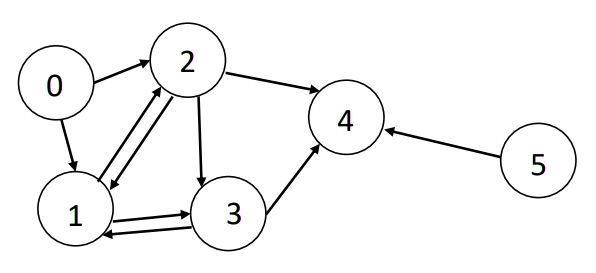
\includegraphics[width=\linewidth]{../pic/python/15.png}
\end{minipage}
Tables , Matrices:\\
\begin{minipage}{0.69\linewidth}
	In general, we can model an $m\times n$ table/matrix using a length-m list L,where L[i] is a length-n list, for i=0,...,m-1
	\begin{itemize}
		\item m = number of rows = len(L)
		\item n = number of columns = row length =len(L[0])
		\item Thus L[i][j] correspond to cell (i,j) in table
	\end{itemize}
\end{minipage}
\begin{minipage}{0.3\linewidth}
	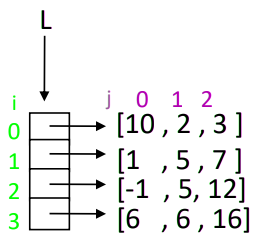
\includegraphics[width=\linewidth]{../pic/python/16}
\end{minipage}
\pagebreak
\subsection{Initializing 2-dimensional list}
Given $m$ and $n$ and a scalar $val$.\\
an $m \times n$ 2-dimensional list L whose entries are all equal to val can be created:
\begin{itemize}
	\item using * operator:
\begin{lstlisting}[language=python]
L = [0]*m 
for i in range(m):
	L[i] = [val]*n
\end{lstlisting}
	\item Compact method using list comprehension
\begin{lstlisting}[language=python]
L = [[val for j in range(n)] for i in range(m)]
\end{lstlisting}
\end{itemize}
\subsection{Printing matrices}
Printing matrices:
{\small\begin{lstlisting}[language=python]
import numpy 
M = [[10,2,3],[1,-500,7],[1,5,12],[6,6,16]]
print(M)
print(numpy.matrix(M))
-----------------------------
OUTPUT: 
[[10,2,3],[1,-500,7],[1,5,12],[6,6,16]]
[[10  2  3]
[1  -500  7]
[1  5  12]
[6  6  16]]
\end{lstlisting}}
Printing a boolean matrices
{\small\begin{lstlisting}[language=python]
M = [[True,False,False],
[False,True,True],
[True,False,True],]
print(numpy.matrix(M))
print(numpy.matrix(M,int))
-----------------------------
OUTPUT: 
[[True False False]
[False True True]
[True False True]]

[[1 0 0]
[0 1 1]
[1 0 1]]
\end{lstlisting}}
\pagebreak
\section{Applications of 2-dimensional lists}
\subsection{Check if given matrix is symmetric}
A matrix M is called symmetric if:
\begin{itemize}
	\item 1. number n of columns = number m of rows
	\item 2. M[i][j] = M[j][i]
\end{itemize}
{\small\begin{lstlisting}[language=python]
def checkIfSymmetric(M):
    m = len(M)
    n = len(M[0])
    if m!=n: return False 
    for i in range(n):
        for j in range(i+1,n):
            if M[i][j] !=M[j][i]
                return False
    return True
\end{lstlisting}}
\subsection{Maze reachability: right-down moves}
$m\times n$ table with True and False entries:
\begin{itemize}
	\item True indicates an open square
	\item False indicates a blocked square
\end{itemize}
Once in an open square, you can possibly move to two squares: \\
the square on the right if it is open and the square below if open.

\begin{center}
	\begin{minipage}{0.3\linewidth}
		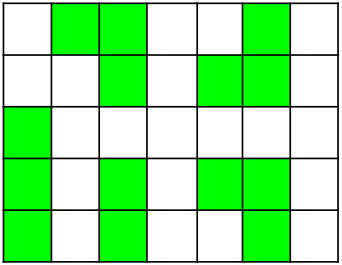
\includegraphics[width=\linewidth]{../pic/python/17}
	\end{minipage}
	\begin{minipage}{0.3\linewidth}
		.
	\end{minipage}
	\begin{minipage}{0.3\linewidth}
		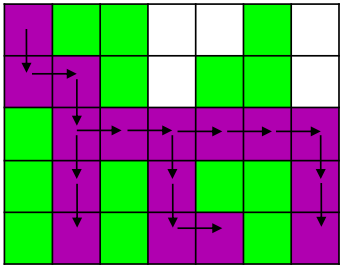
\includegraphics[width=\linewidth]{../pic/python/18}
	\end{minipage}
\end{center}
{\small\begin{lstlisting}[language=python]
def mazeReachableCells(M):
	m = len(M)
	n = len(M[0])
	R = [[False for j in range(n)] for i in range(m)]
	R[0][0] = M[0][0]
	for i in range(m):
		for j in range(n):
			if R[i][j]:
				if i<m-1 and M[i+1][j]:
					R[i+1][j] = True  
				if j<n-1 and M[i][j+1]:
					R[i][j+1] = True 
	return R
\end{lstlisting}}
\section{Dictionaries}
\subsection{Dictionaries}
Dictionary (dict) is a built in type in python. \\
While lists are indexed by integers, dictionaries are indexed by keys.\\
Syntax to definite a new dictionary :
\begin{lstlisting}[language=python]
D = \{ key:value,anotherKey:anotherValue,... \}
\end{lstlisting}
Use subscript operator to access value given key: D[key]
Entries in a dictionary are unordered
\subsection{Dictionary operations}
As a data structure, a dictionary supports the four operations/queries:
\begin{itemize}
	\item Search for key: key in D: return True or False
	\item Access value given key (read/write): D[key] In read mode, gives an error “KeyError: key” if key is not in D
	\item Delete entry given key: del D[key] Gives an error “KeyError: key” if key is not in D
	\item Add new entry (newKey/val pair): D[newKey] = val It overwrites old value if newKey exists in dictionary
\end{itemize}
Dictionaries are mutable.\\
Their values can be mutable objects,but not their keys: keys must be immutable.\\
All 4 dict operations add, access, search, and delete take O(1) time on the average
\subsection{Iterating over keys in dictionaries}
{\small\begin{lstlisting}[language=python]
for key in D: 
	#proccess D[key]
\end{lstlisting}}
\subsection{Copy, clear, update, equality check}
\begin{itemize}
	\item Copy
	      \begin{itemize}
		      \item Assignment operator: D2 = D creates an alias D2 of D
		      \item Copy method dict.copy: D2 = D.copy() : depth-1 only
		      \item Deep copy: copy.deepcopy(D) returns a deep copy (need to import copy)
	      \end{itemize}
	\item Clear: \\
	      To clear all the entries of a dictionary: D.clear()
	      \begin{itemize}
		      \item Not the same as D = {}
		      \item If D has an alias, D.clear() also clears the alias but D = {} doesn’t
	      \end{itemize}
	\item Add: \\
	      To add dictionary D2 to dictionary D: D.update(D2)
	\item equality check:\\
	      To check if two dictionaries D1 and D2 are equal D1 ==D2
\end{itemize}
\section{Applications of dictionaries}
\begin{center}
	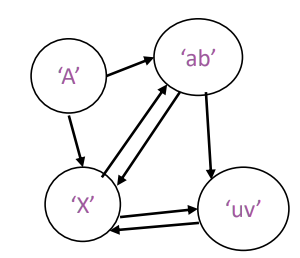
\includegraphics[width=0.3\linewidth]{../pic/python/19.png}
\end{center}
Using Adj to represent graph:
\begin{itemize}
	\item key = node label
	\item value = list of adjacent nodes
\end{itemize}
Adj[s] is a list containing the nodes adjacent to node s: \\
Adj = {'A':['X','ab'],'X':['ab','uv'],'ab':['X','uv'],'uv':['X']}
\subsection{Frequency of words in a file}
{\small\begin{lstlisting}[language=python]
def freqOfWordsInFile(fileName):
    nameHandle = open(fileName, 'r')
    s = nameHandle.read() # read file into a string s
    nameHandle.close()
    L = s.split() # store words in list L
    D = {} # initialize empty dictionary D : keys = words, values= frequencies  
    for w in L:  # loop over strings in list L 
        if w  not in D: # search for w in D
            D[w] = 1 # if not found: add w as a new word with frequency  1  
        else: 
            D[w] +=1 # increment frequency of w if found 
    return D

D = freqOfWordsInFile("findFreqInFile.py")
for w in D:
    print("Word:",w,"   Frequency:",D[w])
\end{lstlisting}}
\subsection{2-SUM}
{\small\begin{lstlisting}[language=python]
def twoSumUsingDictionary(L,t): # O(n) expected time 
    D = {}
    for i in range(len(L)):
        if L[i] not in D: 
            D[L[i]] = i
    for x in L:
        if t-x in D: 
            return (D[x],D[t-x])
    return (-1,-1)
\end{lstlisting}}
\section{Stacks}
We have already seen an example of a stack: the recursion stack
In general, a stack S is a data structure, which as a dynamic set supports operations:
\begin{itemize}
	\item Push object x to stack S
	\item Pop object from stack S and return it: removed object is the last
	\item is stack empty
\end{itemize}
We can use a list S as a stack :
\begin{itemize}
	\item Push: \begin{lstlisting}[language=python]
S.append(x)
\end{lstlisting}
	\item Pop : \begin{lstlisting}[language=python]
S.pop()
\end{lstlisting}
	\item Is stack empty \begin{lstlisting}[language=python]
len(S) == 0
\end{lstlisting}
\end{itemize}

\chapter{Classes and object oriented programming}
\section{Intro}
Objects are collections of data and the methods.\\
Every object has a type, of which the object is an instance.\\

Abstract data type (ADT) is a type of objects with data and associated methods also called operations.
\section{User defined classes}
Syntax to define a class: class keyword:
{\small\begin{lstlisting}[language=python]
class className:
	def method1(..):
		....
	def method2(..):
		....
\end{lstlisting}}
\begin{center}
	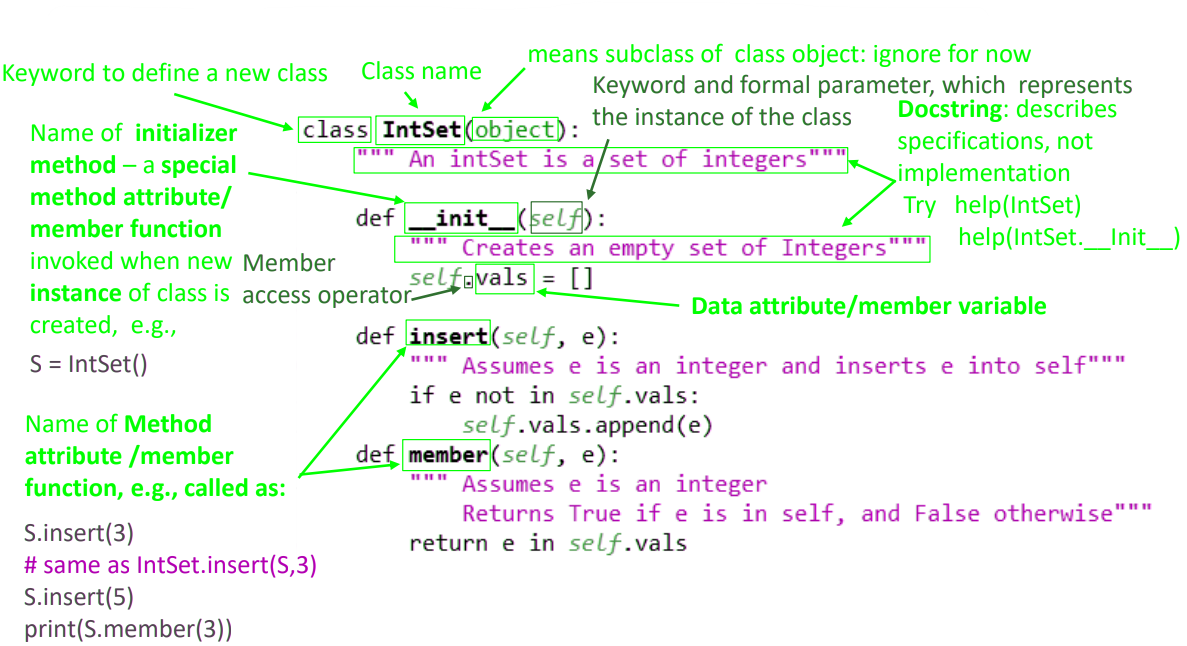
\includegraphics[width=0.8\linewidth]{../pic/python/20.png}
\end{center}
\section{OOP machinery}
\subsection{Terminologies}
\begin{itemize}
	\item Dot operator: used to reference attributes
	\item Attributes/member:
	      \begin{itemize}
		      \item data attribute
		      \item method attribute
	      \end{itemize}
	\item self keyword: if f is a method attribute of a class and S is an instance of the class,calling S.f results in assigning S to self.
	\item Special methods: (start and end with double underscore):
	      \begin{itemize}
		      \item \_\_init\_\_(self,arg1,arg2,...):\\
		            intializer method, invoked when a new instance of the class is created
		      \item \_\_str\_\_(self):\\
		            string representation method invoked by print and str functions
	      \end{itemize}
\end{itemize}
\subsection{Other special methods }
\begin{center}
	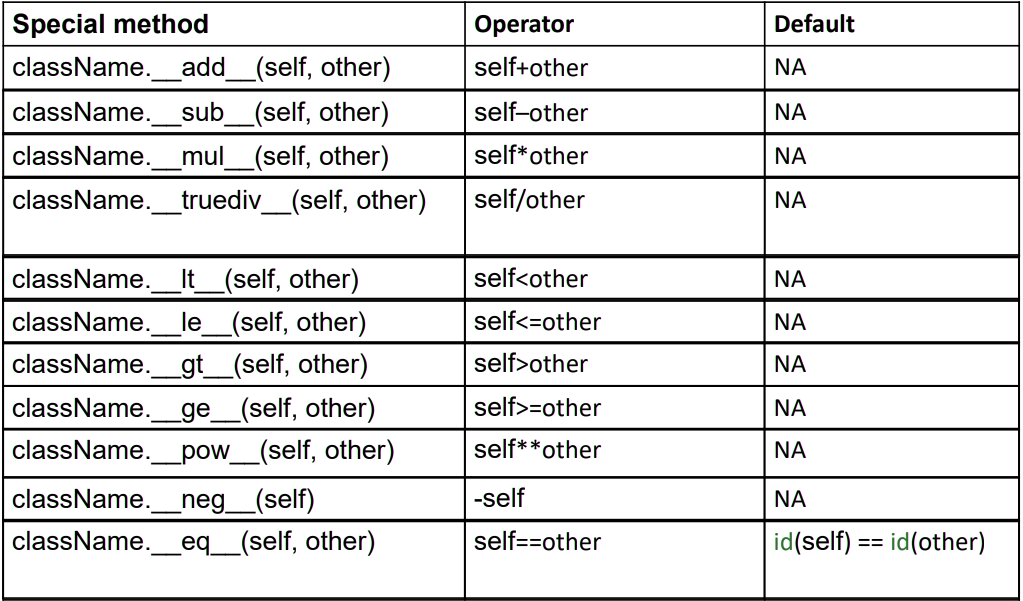
\includegraphics[width=0.8\linewidth]{../pic/python/21.png}
	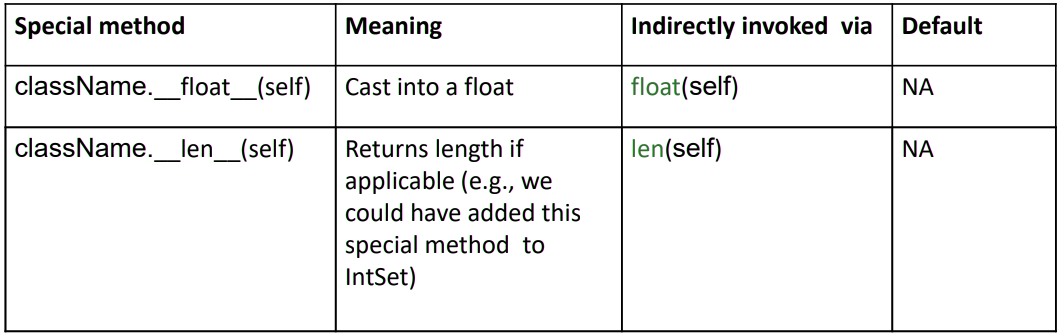
\includegraphics[width=0.8\linewidth]{../pic/python/22.png}
\end{center}
\section{OOP concepts}
\begin{itemize}
	\item \begin{itemize}
		      \item Getters: methods which do not modify data attributes.
		      \item Setters: methods which modify data attributes.
	      \end{itemize}
	\item Encapsulation: It means bundling together data attributes and associated methods attributes
	\item Information hiding:\\
	      Information hiding allows a programmer to change the implementation of the class (e.g., to improve efficiency) without breaking the code that uses the class based on specifications.
\end{itemize}
\section{Inheritance}
Inheritance enables a programmer to define a class in terms of another class.\\
Instead of defining a new class from scratch, a class could be defined as subclass by inheriting certain attributes from a base class.\\
Inheritance gives a hierarchy of types.\\

Syntax to define classB as subclass of classA,i.e.,derive classB from classA:
{\small\begin{lstlisting}[language=python]
class classB(classA):
	def ....
\end{lstlisting}}
The subclass Inherits all attributes (data and methods) of base class.\\
We can override, i.e., replace, method attributes of the base class in the subclass.\\
We can include new attributes in the subclass.
\section{Class variables}
Syntax to define a class variable var :
{\small\begin{lstlisting}[language=python]
class className:
	var = initial value 
	def method ... 
		...
\end{lstlisting}}
to access var: use className.var
\chapter{Stack class derived from list}
\section{Stack}
A stack S is a data structure, which as a dynamic set supports operations:
\begin{itemize}
	\item Push
	\item Pop
	\item is empty?
\end{itemize}
{\small\begin{lstlisting}[language=python]
class Stack(list):
    """ class Stack derived from list"""
    def push(self,value):
        self.append(value)
    def top(self):
        assert not self.isEmpty(), "Stack Empty!"
        return self[len(self)-1]
    def isEmpty(self):
        return (len(self)==0)
            \end{lstlisting}}
Pop and Push operations take O(1) amortized time
\section{Queue}
Queues are like stacks except that the removed object is the first in instead of last in\\
A queue Q is a data structure, which as a dynamic set supports operations:
\begin{itemize}
	\item Enqueue
	\item Dequeue
	\item is queue empty
\end{itemize}
\pagebreak
\subsection{Non-efficient implementation}
Similarly to a stack, could implement it using a list Q:
\begin{itemize}
	\item Enqueue: Q.append(x)
	\item Dequeue: Q.pop(0)
	\item is empty : len(Q) ==0
\end{itemize}
The issue is Q.pop(0) takes O(len(Q)) time
\subsection{Wrap-around}
\begin{minipage}{0.5\linewidth}
	\begin{itemize}
		\item Use Data attributes:
		      \begin{itemize}
			      \item maxSize
			      \item List L of length maxSize
			      \item size: number of elements in queue
			      \item tail: index in L
			      \item head: index in L
		      \end{itemize}
		\item \_\_init\_\_ method:
		      \begin{itemize}
			      \item takes maxSize as input argument and initializes L
		      \end{itemize}
		\item enqueue method:
		      \begin{itemize}
			      \item check if full
			      \item insert element at the tail
			      \item increment tail in a circular fashion
			      \item increment size
		      \end{itemize}
		\item dequeue method:
		      \begin{itemize}
			      \item check if empty
			      \item read value at head
			      \item increment head in a circular fashion
			      \item return value
		      \end{itemize}
		\item Other methods :
		      \begin{itemize}
			      \item peakHead(return value at head)
			      \item isFull,isEmpty
			      \item \_\_str\_\_,\_\_len\_\_(return size)
		      \end{itemize}
	\end{itemize}

\end{minipage}
\begin{minipage}{0.4\linewidth}
	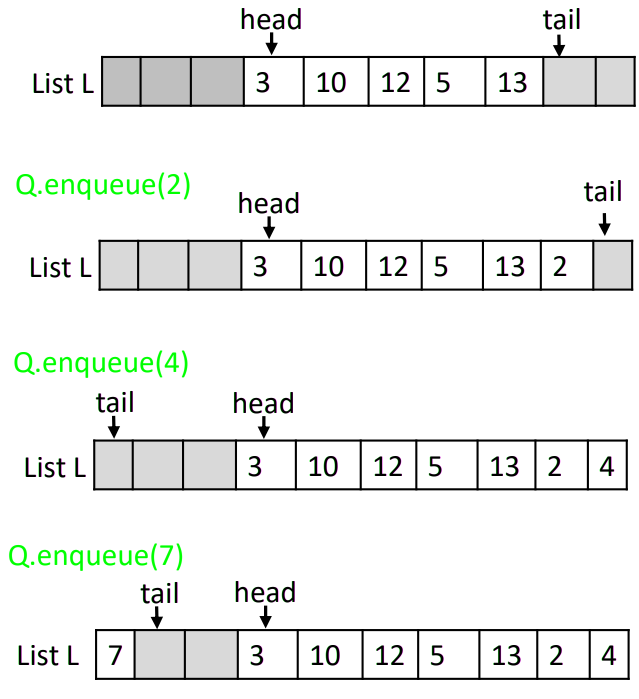
\includegraphics[width=\linewidth]{../pic/python/23}\\
	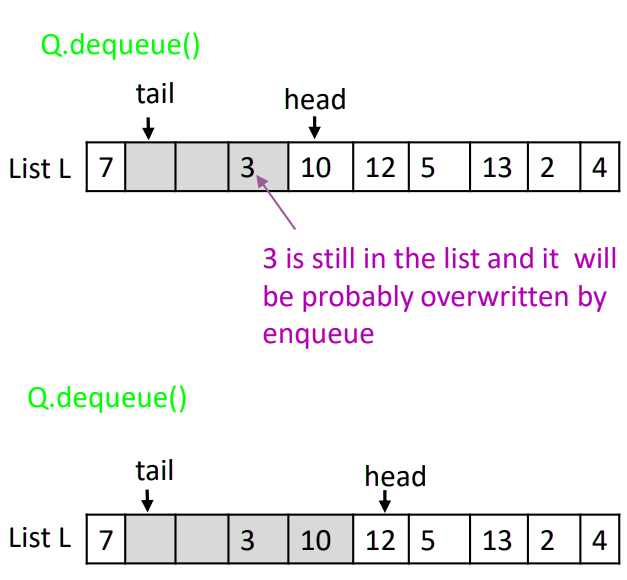
\includegraphics[width=\linewidth]{../pic/python/24}
\end{minipage}
\pagebreak
{\small\begin{lstlisting}[language=python]
class Queue(object):
    """ Queue with given max size """ 
    def __init__(self, maxSize=10):
        """ takes maxSize whose  default value is 10 """
        self.L = [None]*maxSize
        self.size = 0
        self.maxSize = maxSize
        self.tail = 0
        self.head = 0
    def enqueue(self,value):
        """ adds value to queue, raises exception if full """ 
        assert not self.isFull(), "Queue Full"
        self.L[self.tail]=value
        if self.tail<self.maxSize-1:
            self.tail+=1
        else: 
            self.tail = 0
        self.size+=1
    def dequeue(self):
        """ removes and returns first value in, raises exception if empty"""
        assert not self.isEmpty(), "Queue Empty"         
        val = self.L[self.head]
        if self.head<self.maxSize-1:
            self.head+=1
        else: 
            self.head=0
        self.size-=1         
        return val 
    def peakHead(self):
        """ returns value at head, raises exception if empty"""
        assert not self.isEmpty(), "Queue Empty"   
        return self.L[self.head] 
    def isFull(self):
        """ returns True if full"""
        return self.size==self.maxSize 
    def isEmpty(self):
        """ returns True if empty"""        
        return self.size==0
    def __str__(self):
        """represent elements in queue as a string:
           separated by commas and between brackets"""
        s = "["
        index  = self.head 
        for count in range(self.size): 
            s = s+ str(self.L[index])+","
            if index<self.maxSize-1:
                index+=1
            else: 
                index=0
        return s[:-1]+"]"
        # -1 to remove the trailing comma 
    def __len__(self):
        return self.size 
\end{lstlisting}}
\subsubsection{Drawbacks and improvement}
\begin{itemize}
	\item One drawback: need to set maxSize at initialization and live with it. \\
	      Solution: 
	      \begin{itemize}
		      \item Double list size if maxSize reached
	      \end{itemize}
	\item Another drawback which has a similar solution is that too much space remains reserved if queue grows a lot and then shrinks a lot.
\end{itemize}

\end{document}